\documentclass{article}
\usepackage{graphicx}
\graphicspath{ {../diagram/} }
\usepackage[margin=2cm]{geometry}
\usepackage{enumitem}
\usepackage{caption}
\usepackage{subcaption}
\usepackage{amsmath}
\usepackage{booktabs}
\usepackage{multirow}
\newcommand{\qaS}{0}
\newcommand{\qaE}{1000\_1011}
\newcommand{\qaF}{0000\_011}
\newcommand{\qaDecim}{$4192$}
\newcommand{\qbS}{0}
\newcommand{\qbE}{0000\_0000}
\newcommand{\qbF}{0000\_000}
\newcommand{\qbDecim}{$0$}
\newcommand{\qcS}{0}
\newcommand{\qcE}{0000\_0000}
\newcommand{\qcF}{0000\_000}
\newcommand{\qcDecim}{$0$}
\newcommand{\qdS}{0}
\newcommand{\qdE}{0111\_1000}
\newcommand{\qdF}{0010\_001}
\newcommand{\qdDecim}{$0.00885009765625$}


\title{DSP in VLSI \\ Homework 3 - Interpolator}
\author{Jen-Tse Chen}
\date{April 2026}

\begin{document}
\maketitle

\begin{enumerate}

    \item (Step 1) Show the real-part and imaginary-part output waveform $\hat{x}_1[m+\mu]$ after interpolation using linear interpolator and second-order polynomial interpolator to interpolate the sampled waveform in the region of $10 \leq m \leq 20$ with $\mu = 0, \frac{1}{8}, \frac{2}{8}, \ldots\frac{7}{8}$. In addition, draw the absolute error, defined by $|x_1[m+\mu] - \hat{x}_1[m+\mu]|$ in the region of $10 \leq m \leq 20$ with $\mu = 0, \frac{1}{8}, \frac{2}{8}, \ldots\frac{7}{8}$. (30\%)

    Figure \ref{fig:x1_interp} shows the interpolated waveform and the absolute error of the linear and second-order polynomial interpolators for $x_1[m+\mu]$.

    \begin{figure}[htbp]
        \centering
        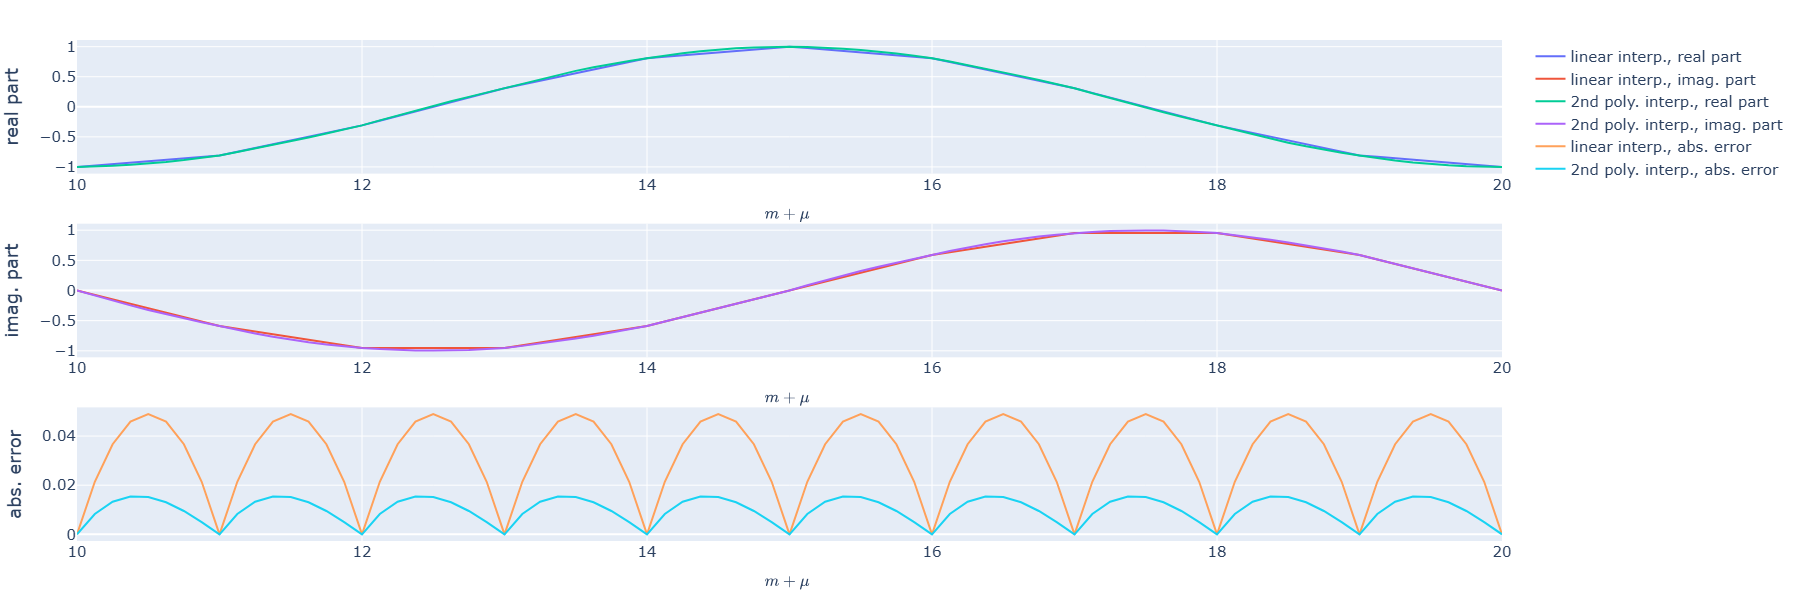
\includegraphics[width=1.0\textwidth]{../diagram/Q1/x1_interp.png}
        \caption{Interpolated waveform and absolute error of $\hat{x}_1[m+\mu]$}
        \label{fig:x1_interp}
    \end{figure}

    \newpage
    \item (Step 2) Show the real-part and imaginary-part output waveform of $\hat{x}_2[m+\mu]$ after interpolation using linear interpolator and piecewise parabolic interpolator to interpolate the sampled waveform in the region of $5 \leq m \leq 10$ with $\mu = 0, \frac{1}{9}, \frac{2}{9}, \ldots\frac{8}{9}$. In addition, draw the absolute error, defined by $|x_2[m+\mu] - \hat{x}_2[m+\mu]|$ in the region of $4 \leq m \leq 8$ with $\mu = 0, \frac{1}{8}, \frac{2}{8}, \ldots\frac{7}{8}$. (30\%)

    Figure \ref{fig:x2_interp} shows the interpolated waveform and the absolute error of the linear and piecewise parabolic interpolators for $x_2[m+\mu]$.

    \begin{figure}[htbp]
        \centering
        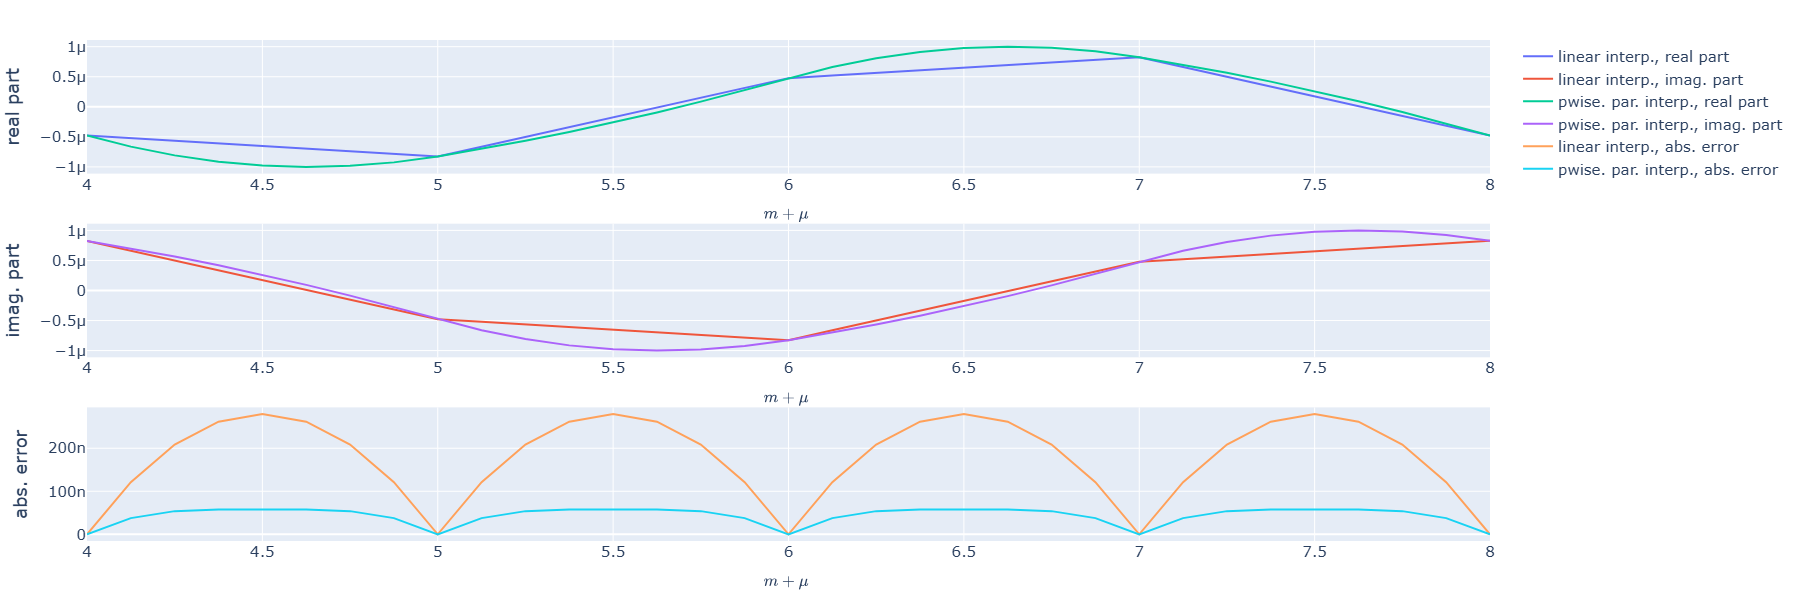
\includegraphics[width=1.0\textwidth]{../diagram/Q2/x2_interp.png}
        \caption{Interpolated waveform and absolute error of $\hat{x}_2[m+\mu]$}
        \label{fig:x2_interp}
    \end{figure}

    \item (Step 3) Please show the results calculated by your BF16 bit-true model for the following operands and operators. Express results both in decimal and binary representation. (S, E, F mean the sign bit, exponent field, and fraction field. All are given in binary.) (20\%)

    \begin{table}[htbp]
        \centering
        \begin{tabular}{|l|l|l|l|l|l|}
            \hline
            & \textbf{Operand 1} & \textbf{Operand 2} & \textbf{Operation} & \textbf{Result (Binary)}  & \textbf{Result (Decimal)} \\
            \hline
            \multirow{3}{*}{(a)} & S: 1             & S: 0             & \multirow{3}{*}{Addition}       & S: \qaS & \multirow{3}{*}{\qaDecim} \\
                                 & E: 1000\_0011    & E: 1000\_1011    &                                 & E: \qaE & \\
                                 & F: 0000\_000     & F: 0000\_011     &                                 & F: \qaF & \\
            \hline
            \multirow{3}{*}{(b)} & S: 1             & S: 0             & \multirow{3}{*}{Addition}       & S: \qbS & \multirow{3}{*}{\qbDecim} \\
                                 & E: 0000\_0001    & E: 0000\_0001    &                                 & E: \qbE & \\
                                 & F: 0000\_011     & F: 1111\_010     &                                 & F: \qbF & \\
            \hline
            \multirow{3}{*}{(c)} & S: 1             & S: 0             & \multirow{3}{*}{Multiplication} & S: \qcS & \multirow{3}{*}{\qcDecim} \\
                                 & E: 0000\_0010    & E: 0111\_1100    &                                 & E: \qcE & \\
                                 & F: 1100\_000     & F: 0000\_110     &                                 & F: \qcF & \\
            \hline
            \multirow{3}{*}{(d)} & S: 0             & S: 0             & \multirow{3}{*}{Multiplication} & S: \qdS & \multirow{3}{*}{\qdDecim} \\
                                 & E: 0110\_0011    & E: 1001\_0011    &                                 & E: \qdE & \\
                                 & F: 1011\_110     & F: 0101\_000     &                                 & F: \qdF & \\
            \hline
        \end{tabular}
        \caption{BF16 bit-true model computation results}
        \label{table:bf16_results}
    \end{table}

    \newpage
    \item (Step 4) Show the interpolation differences of the second-order interpolator using BF16 and double-precision arithmetic operations. Draw the figures indicating the difference of interpolated results caused by data format for outputs $\hat{x}_1[m+\mu]$ in the region of $10 \leq m \leq 20$ with $\mu = 0, \frac{1}{8}, \frac{2}{8}, \ldots\frac{7}{8}$. (10\%)

    Figure \ref{fig:x1_poly2_bf16_diff} shows the interpolated waveform of $\hat{x}_1[m+\mu]$ using double-precision and BF16 arithmetic, and the absolute difference between the two results caused by the finite precision of BF16.

    \begin{figure}[htbp]
        \centering
        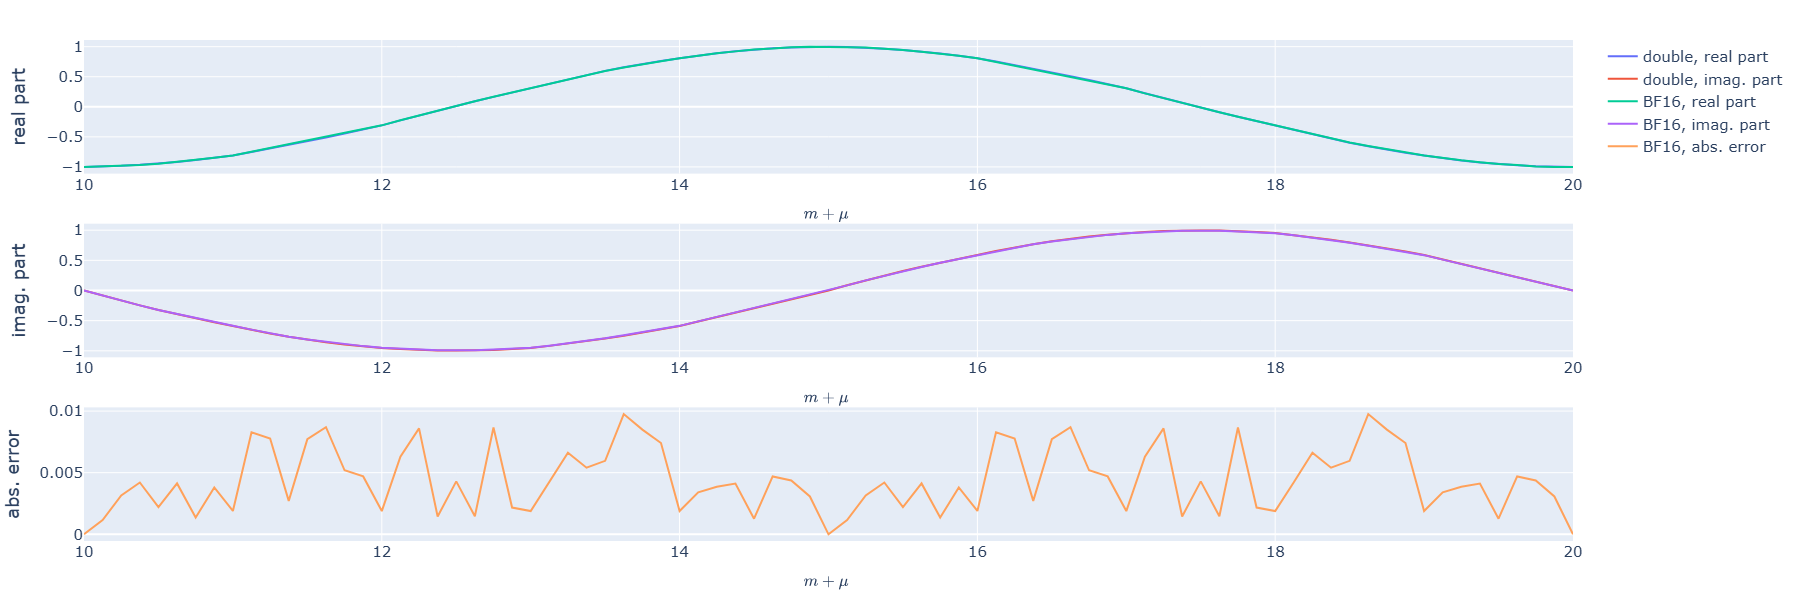
\includegraphics[width=1.0\textwidth]{../diagram/Q4/x1_poly2_bf16_diff.png}
        \caption{Interpolated waveform and absolute error of $\hat{x}_1[m+\mu]$ between double-precision and BF16}
        \label{fig:x1_poly2_bf16_diff}
    \end{figure}

    \newpage
    \item (Step 5) Draw the complete block diagram of your first version implementation according to the Farrow structure. (5\%) Show your hardware sharing version (the precision of the datapath must be BF16 and cannot be changed). (10\%) Draw the block diagram after your improvement. (5\%) Indicate the critical path. (5\%)

    Answer text here.

    \newpage
    \item (Step 6) Write HDL to implement your second-order interpolator using BF16 arithmetic unit of Farrow structure after reduction. The input to be interpolated will change every 8 clock cycles and $\mu$ will change every clock cycle. Show the timing diagram of behavior simulation for the first 8 ($\mu = 0, \frac{1}{8}, \frac{2}{8}, \ldots\frac{7}{8}$) and the last 8 ($\mu = 0, \frac{1}{8}, \frac{2}{8}, \ldots\frac{7}{8}$) interpolated outputs of $\hat{x}_1[m+\mu]$ in the region of $10 \leq m \leq 20$. Show the real-part and imaginary-part error compared to double-precision results. (30\%)

    Answer text here.

    \newpage
    \item (Step 6) Show your timing report to verify the critical path of your block diagram in Q5. (10\%) List your timing constraint for post-synthesis simulation. (5\%)

    Answer text here.

    \newpage
    \item (Step 6) Show the timing diagram of post-synthesis simulation for the first 8 ($\mu = 0, \frac{1}{8}, \frac{2}{8}, \ldots\frac{7}{8}$) and the last 8 ($\mu = 0, \frac{1}{8}, \frac{2}{8}, \ldots\frac{7}{8}$) interpolated outputs of $\hat{x}_1[m+\mu]$ in the region of $10 \leq m \leq 20$ with $\mu = 0, \frac{1}{8}, \frac{2}{8}, \ldots\frac{7}{8}$. Show the real-part and imaginary-part error compared to double-precision results. (20\%)

    Answer text here.

    \newpage
    \item (Step 6) Construct your BF16 bit-true model as the architecture after your improvement. Depict the real-part and imaginary-part errors of interpolated outputs of $\hat{x}_1[m+\mu]$ between the Verilog outputs and the bit-true model in the region of $10 \leq m \leq 20$ with $\mu = 0, \frac{1}{8}, \frac{2}{8}, \ldots\frac{7}{8}$. (20\%)

    Answer text here.

\end{enumerate}

\end{document}
